\chapter{Introduction}
\label{ch:intro}

\begin{figure}[t]
  \centering
  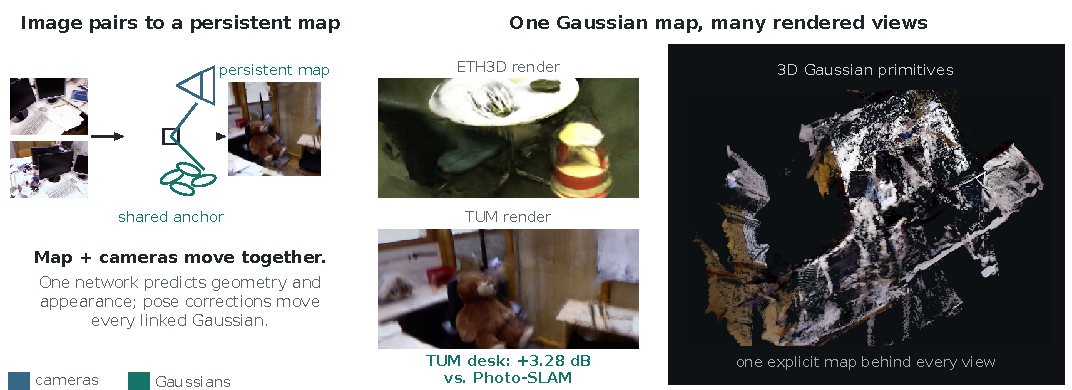
\includegraphics[width=\linewidth]{ral/fig/teaser.pdf}
  \caption[From local predictions to a persistent map]{Splatt3R-SLAM
  predicts local Gaussian maps, carries them with keyframe anchors, and
  refines their appearance. The image is a middle-ranked Replica office0
  comparison. The chart reports all eight Replica scenes with common
  non-keyframe cameras and full exported SH.}
  \label{fig:teaser}
\end{figure}

A robot map must remain useful after the camera has left a room. It must
support localisation, preserve scene structure, and show what the scene
looks like from another viewpoint. Classical visual SLAM provides camera
motion and geometry. 3D Gaussian splatting~\cite{kerbl20233dgs} adds a
renderable appearance model.

Most Gaussian SLAM systems build this model through per-scene optimisation.
MonoGS~\cite{matsuki2024monogs}, Photo-SLAM~\cite{huang2024photoslam}, and
related systems create and update primitives as images arrive.
Feed-forward reconstruction offers another starting point.
DUSt3R~\cite{wang2024dust3r} and MASt3R~\cite{leroy2024mast3r} predict dense
geometry from image pairs. Splatt3R~\cite{smart2024splatt3r} extends the same
features with Gaussian position, shape, colour, and opacity.

This pairwise capability changes the cost of map creation, but it leaves a
sequence-level problem. Every image pair defines a local coordinate frame.
Repeated observations create overlapping copies of the same surface.
Later loop closures move earlier camera poses. Simply concatenating the
predictions therefore produces a large map whose placement and appearance
can become inconsistent.

\section{The central idea}

Splatt3R-SLAM gives every local map a keyframe anchor. Its Gaussians remain
in that anchor's coordinates and move when the pose graph updates the
keyframe. The images used to refine the map are stored relative to the same
anchors. A pose correction then moves the local map and its observation
cameras together.

This shared-anchor relation is the thread through the thesis. It connects
pairwise prediction to a persistent map, allows appearance refinement to
run after tracking, and gives each experiment a clear role. The system
follows three stages:
\begin{enumerate}\itemsep3pt
\item \textbf{Predict} a local Gaussian map from an image pair.
\item \textbf{Anchor} the map and its supervision to the pose graph.
\item \textbf{Refine} Gaussian appearance against tracked RGB observations.
\end{enumerate}
The geometric tracker remains MASt3R-SLAM~\cite{murai2025mast3rslam}.
The mapping process reads its poses but does not optimise them.

\section{Research questions}
\label{sec:intro:rq}

The experiments address four questions:
\begin{description}\itemsep4pt
\item[RQ1] How can pairwise Gaussian prediction be adapted without changing
the shared geometric features used for tracking?
\item[RQ2] Can opacity attenuation at insertion reduce the effect of
overlapping predictions in an assembled map?
\item[RQ3] How much appearance improvement comes from sequence-level
refinement, and can it be delivered without disrupting tracking?
\item[RQ4] How does the complete system compare with locally executed SLAM
baselines in rendering quality, trajectory accuracy, map size, and compute?
\end{description}

\section{From design to evidence}

Each chapter tests one part of the pipeline. Head-only adaptation changes
the first stage while the encoder and decoder stay frozen. Opacity thinning
changes the second stage by lowering the initial contribution of selected
primitives. The refiner changes the third stage through an RGB rendering
loss. Paired studies isolate these interventions before the complete system
is compared with other methods.

The main external result uses the released Splatt3R head, no thinning,
fixed Gaussian centres, and $300$\,s post-sequence refinement. Under common
non-keyframe reconstruction evaluation, its mean PSNR on eight Replica
scenes is $23.02$\,dB, compared with $19.48$\,dB for Photo-SLAM.
On TUM desk, its $13.95$\,dB is close to MonoGS's $13.91$\,dB, while
MonoGS has lower LPIPS. The same evaluation also exposes the cost of dense
prediction: the TUM map contains $2.397$ million primitives.

\section{Contributions}
\label{sec:intro:contrib}

\begin{enumerate}\itemsep4pt
\item A pose-anchored mapping design in which local Gaussians and their
supervision cameras follow the same keyframe corrections
(\cref{ch:system,ch:refiner}).
\item A decoupled refinement process that improves appearance without
updating the tracking model or camera poses, with causal, latency, and
two-GPU controls (\cref{ch:refiner,ch:results}).
\item Paired studies of head-only adaptation and insertion-time opacity
attenuation, including controls for confidence weighting and refinement
(\cref{ch:adapt,ch:thin}).
\item Common-camera reconstruction comparisons with all-eight-scene Replica
coverage, four-method qualitative views, trajectory controls, and explicit
map-size and resource measurements (\cref{ch:protocol,ch:results}).
\end{enumerate}

\section{Thesis structure}

\Cref{ch:bg,ch:related} introduce Gaussian rendering, pairwise prediction,
and related SLAM systems. \Cref{ch:system} presents the shared-anchor design.
\Cref{ch:adapt,ch:thin,ch:refiner} explain the three intervention stages.
\Cref{ch:protocol,ch:results} define and report the evaluation.
\Cref{ch:negative} records tested routes that did not improve the complete
system. \Cref{ch:discussion,ch:conclusion} discuss the remaining problems
and future work. The appendices contain configurations, reproduction steps,
baseline build records, and extended tables.
